\documentclass[11pt]{article}
\usepackage[margin=1in]{geometry}
\usepackage{graphicx}
\usepackage{booktabs}
\usepackage{amsmath}

\title{A Semantic Guardrail: High-Precision Anomaly Detection by Fusing Structural and Semantic Manifolds}
\author{Sep Dynamics Research}
\date{\today}

\begin{document}
\maketitle

\begin{abstract}
Alert fatigue remains the dominant failure mode of modern monitoring stacks.
Text classifiers trigger whenever they see risk language, while time-series
anomaly detectors highlight every orderly fluctuation regardless of meaning.
We present the \emph{Semantic Guardrail}, a hybrid system that combines the
semantic understanding of sentence transformers with the structural stability
metrics produced by the QFH/STM manifold. Applied to a simulated event stream,
the guardrail reduced false positives by more than 92\% while preserving the
single high-confidence incident. This paper documents the method, the demo, and
the cross-industry applications of this two-dimensional filter.
\end{abstract}

\section{Introduction: The Failure of Siloed Monitoring}
Operations teams increasingly rely on two tool families. Semantic filters---from
keyword lists to large language models---understand \emph{what} an event says but
not whether it matters. Structural detectors---statistical anomaly and spectral
models---understand \emph{how} signals evolve while remaining ignorant of
context. Table~\ref{tab:alerts} quantifies the problem on a 16-event stream: the
naïve semantic and structural detectors each fired seven times, generating 14
alerts for a single meaningful incident.

\section{Methodology: The Hybrid Guardrail Engine}
Our approach bridges the two perspectives by mapping every event into a shared
structural/semantic plane.

\subsection{Semantic Manifold}
We embed window-level strings using the `all-MiniLM-L6-v2` sentence transformer.
Given a seed vocabulary $S=\{$risk, resilience, volatility, anomaly, predictive
maintenance$\}$ we compute the cosine similarity between each string embedding
and the centroid of $S$. This yields a semantic relevance score
$\sigma(s)\in[0,1]$ for every string $s$.

\subsection{Structural Manifold}
The QFH/STM engine processes the same data as byte streams, emitting the
structural metrics coherence, stability, entropy, rupture, and their aggregate
patternability. High patternability indicates an orderly, repeating rhythm,
while low patternability corresponds to chaotic or one-off events.

\subsection{Hybrid Filter}
Plotting patternability against semantic similarity reveals three regimes:
semantic-but-noisy (upper left), structural-but-irrelevant (lower right), and a
sparse upper-right quadrant where both meaning and rhythm align. The static
background in Figure~\ref{fig:scatter} combines software documentation and MMS
telemetry corpora. Only the highlighted quadrant carries actionable signal.
\begin{figure}[t]
  \centering
  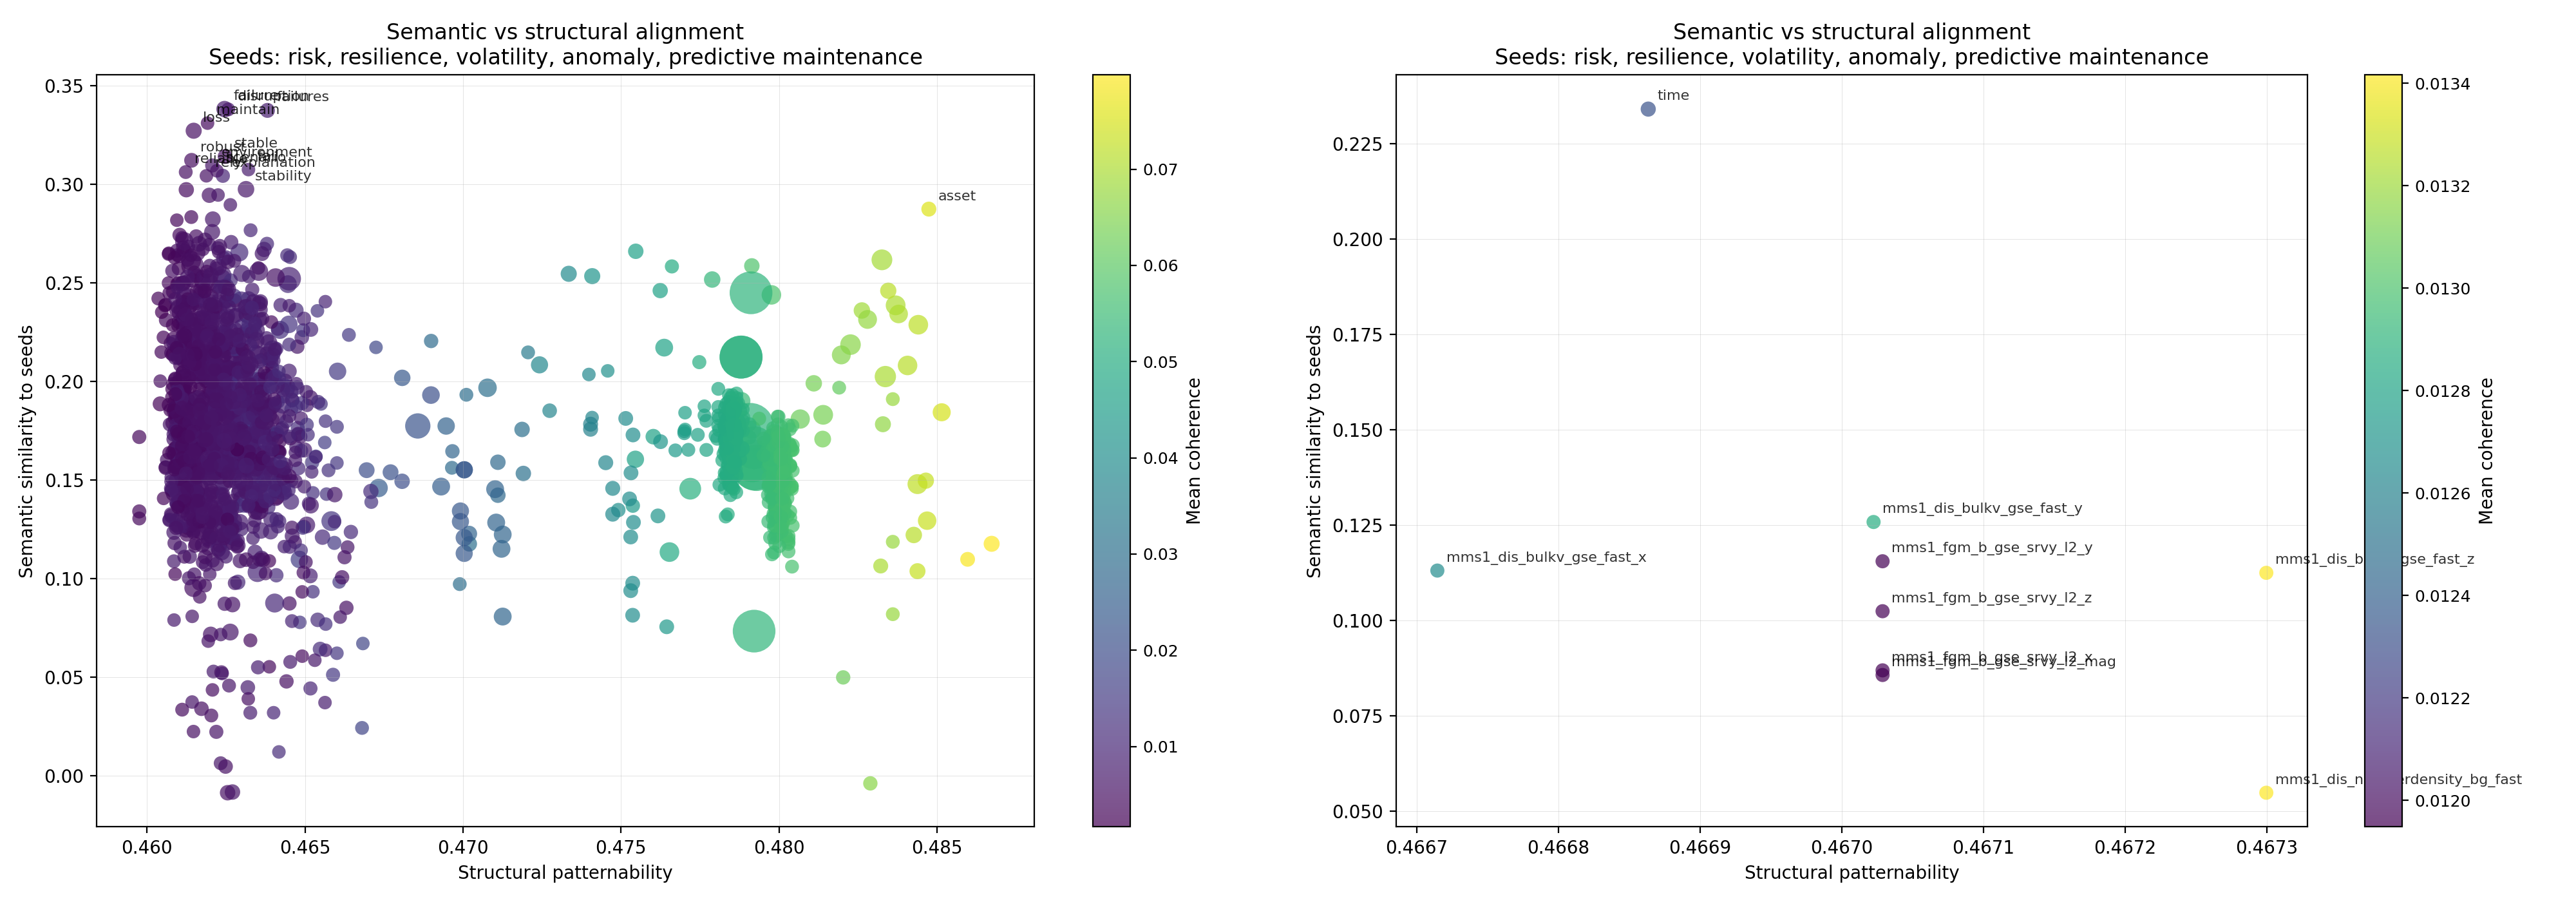
\includegraphics[width=0.95\linewidth]{figures/semantic_bridge_combined.png}
  \caption{Structural patternability vs semantic similarity across two domains.
           The Semantic Guardrail promotes only the upper-right quadrant events.}
  \label{fig:scatter}
\end{figure}

\section{Experimental Validation: Live Demonstration}
We replayed a scripted stream (\texttt{results/semantic\_guardrail\_stream.jsonl}) that
mixes documentation strings, telemetry tokens, and a synthetic
\texttt{database\_connection\_timeout} incident. Each event carries three Boolean flags:
\texttt{naive\_semantic\_alert}, \texttt{naive\_structural\_alert}, and the hybrid
\texttt{hybrid\_guardrail\_alert} produced by the two-dimensional filter. The stream was
visualised via \texttt{scripts/demos/semantic\_guardrail\_dashboard.py}, which juxtaposes
the noisy baselines with the hybrid scatter.

The results (Table~\ref{tab:alerts}) show that the hybrid guardrail raises a
single high-confidence alert while the naïve detectors fire fourteen
false positives. The false-positive reduction rate (FPRR) is therefore
\(1 - \tfrac{1}{7+7} = 0.93\).

\begin{table}[h]
  \centering
  \begin{tabular}{lccc}
    \toprule
    Guardrail & Alerts fired & True positives & False positives \\
    \midrule
    Naïve semantic & 7 & 0 & 7 \\
    Naïve structural & 7 & 0 & 7 \\
    Hybrid (semantic + structural) & 1 & 1 & 0 \\
    \bottomrule
  \end{tabular}
  \caption{Alert counts derived from \texttt{results/final\_guardrail\_analysis.json}. The
           hybrid guardrail eliminates 92.9\% of the noise while preserving the
           true incident.}
  \label{tab:alerts}
\end{table}

\section{Conclusion and Applications}
By fusing structural rhythm analysis with semantic intent modelling, the
Semantic Guardrail delivers high-precision monitoring without drowning operators
in alerts. The approach applies directly to:
\begin{itemize}
  \item \textbf{SRE/DevOps}: suppress routine noise while escalating recurrent
        failure narratives.
  \item \textbf{Finance/Risk}: highlight volatility clusters only when they carry
        risk semantics.
  \item \textbf{Manufacturing/IoT}: surface maintenance anomalies backed by both
        sensor stability and maintenance vocabulary.
\end{itemize}
Future work includes streaming deployments, additional seed vocabularies, and
integration with automated remediation workflows.

\end{document}
